%(BEGIN_QUESTION)
% Copyright 2010, Tony R. Kuphaldt, released under the Creative Commons Attribution License (v 1.0)
% This means you may do almost anything with this work of mine, so long as you give me proper credit

Anta at du skal feilsøke en volumfortrengningsmåler med pulsutgang (én puls per 20 gallon), koblet til en elektronisk teller som summerer total vannflow over tid. Telleren krever et {\it pulserende} signal for å telle opp (stabil ``lav'' eller stabil ``høy'' gir ingen økning), og av en eller annen grunn teller den ikke riktig selv om vi vet at det går vann gjennom flowmåleren. Med digitalt multimeter måler du konstant 0 volt mellom terminalene {\bf J} og {\bf K}, mens du venter lenge nok til at flowmålerbryteren skal ha pulset minst én gang:

$$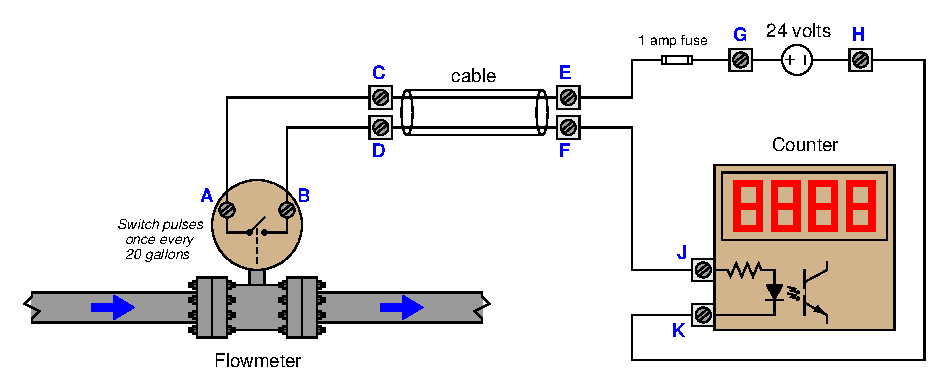
\includegraphics[width=15.5cm]{i00372x01.eps}$$

Vurder sannsynligheten for hver oppgitt feil i kretsen. Se på én feil om gangen (ingen sammenfallende feil), og avgjør om hver feil alene kan forklare {\it alle} målinger og symptomer.

% No blank lines allowed between lines of an \halign structure!
% I use comments (%) instead, so that TeX doesn't choke.

$$\vbox{\offinterlineskip
\halign{\strut
\vrule \quad\hfil # \ \hfil & 
\vrule \quad\hfil # \ \hfil & 
\vrule \quad\hfil # \ \hfil \vrule \cr
\noalign{\hrule}
%
% First row
{\bf Feil} & {\bf Mulig} & {\bf Umulig} \cr
%
\noalign{\hrule}
%
% Another row
Flowmålerbryter har brudd &  &  \cr
%
\noalign{\hrule}
%
% Another row
Sikring gått (brudd) &  &  \cr
%
\noalign{\hrule}
%
% Another row
Brudd i kabel mellom C/D og E/F &  &  \cr
%
\noalign{\hrule}
%
% Another row
Motstand i teller har brudd &  &  \cr
%
\noalign{\hrule}
%
% Another row
Flowmålerbryter er kortsluttet &  &  \cr
%
\noalign{\hrule}
%
% Another row
Kortsluttet kabel mellom C/D og E/F &  &  \cr
%
\noalign{\hrule}
%
% Another row
LED i teller er kortsluttet &  &  \cr
%
\noalign{\hrule}
%
% Another row
Spenningskilde er død &  &  \cr
%
\noalign{\hrule}
} % End of \halign 
}$$ % End of \vbox

\underbar{file i00372}
%(END_QUESTION)





%(BEGIN_ANSWER)

% No blank lines allowed between lines of an \halign structure!
% I use comments (%) instead, so that TeX doesn't choke.

$$\vbox{\offinterlineskip
\halign{\strut
\vrule \quad\hfil # \ \hfil & 
\vrule \quad\hfil # \ \hfil & 
\vrule \quad\hfil # \ \hfil \vrule \cr
\noalign{\hrule}
%
% First row
{\bf Feil} & {\bf Mulig} & {\bf Umulig} \cr
%
\noalign{\hrule}
%
% Another row
Flowmålerbryter har brudd & $\surd$ &  \cr
%
\noalign{\hrule}
%
% Another row
Sikring gått (brudd) & $\surd$ &  \cr
%
\noalign{\hrule}
%
% Another row
Brudd i kabel mellom C/D og E/F & $\surd$ &  \cr
%
\noalign{\hrule}
%
% Another row
Motstand i teller har brudd &  & $\surd$ \cr
%
\noalign{\hrule}
%
% Another row
Flowmålerbryter er kortsluttet &  & $\surd$ \cr
%
\noalign{\hrule}
%
% Another row
Kortsluttet kabel mellom C/D og E/F &  & $\surd$ \cr
%
\noalign{\hrule}
%
% Another row
LED i teller er kortsluttet &  & $\surd$ \cr
%
\noalign{\hrule}
%
% Another row
Spenningskilde er død & $\surd$ &  \cr
%
\noalign{\hrule}
} % End of \halign 
}$$ % End of \vbox


%(END_ANSWER)





%(BEGIN_NOTES)

{\bf Denne oppgaven er ment for eksamen og ikke for arbeidsark!}.

%(END_NOTES)
